% ****** Start of file template.aps ****** %
%%
%%
%%   This file is part of the APS files in the REVTeX 4 distribution.
%%   Version 4.0 of REVTeX, August 2001
%%
%%
%%   Copyright (c) 2001 The American Physical Society.
%%
%%   See the REVTeX 4 README file for restrictions and more information.
%%
%
% This is a template for producing manuscripts for use with REVTEX 4.0
% Copy this file to another name and then work on that file.
% That way, you always have this original template file to use.
%
% Group addresses by affiliation; use superscriptaddress for long
% author lists, or if there are many overlapping affiliations.
% For Phys. Rev. appearance, change preprint to twocolumn.
% Choose pra, prb, prc, prd, pre, prl, prstab, or rmp for journal
%  Add 'draft' option to mark overfull boxes with black boxes
%  Add 'showpacs' option to make PACS codes appear
%  Add 'showkeys' option to make keywords appear
\documentclass{revtex4}
%\documentclass[aps,prl,preprint,superscriptaddress]{revtex4}
%\documentclass[aps,prl,twocolumn,groupedaddress]{revtex4}
\usepackage[dvipdf]{graphicx}
\usepackage{amsmath}
\usepackage{amssymb}
\usepackage{hyperref}
%\usepackage{dcolumn}

% You should use BibTeX and apsrev.bst for references
% Choosing a journal automatically selects the correct APS
% BibTeX style file (bst file), so only uncomment the line
% below if necessary.
%\bibliographystyle{apsrev}

\begin{document}

% Use the \preprint command to place your local institutional report
% number in the upper righthand corner of the title page in preprint mode.
% Multiple \preprint commands are allowed.
% Use the 'preprintnumbers' class option to override journal defaults
% to display numbers if necessary
%\preprint{}

%Title of paper
\title{Precise Measurement of Local Gravitational Acceleration
with a Reversible Pendulum}

% repeat the \author .. \affiliation  etc. as needed
% \email, \thanks, \homepage, \altaffiliation all apply to the current
% author. Explanatory text should go in the []'s, actual e-mail
% address or url should go in the {}'s for \email and \homepage.
% Please use the appropriate macro foreach each type of information

% \affiliation command applies to all authors since the last
% \affiliation command. The \affiliation command should follow the
% other information
% \affiliation can be followed by \email, \homepage, \thanks as well.
\author{Physics 2501: Mechanics and Electromagnetism Laboratory}
%\homepage[]{Your web page}
%\thanks{}
%\altaffiliation{}
\affiliation{Dept. of Physics, University of Connecticut}
%\author{R.T. Jones}
%\affiliation{University of Connecticut}

%Collaboration name if desired (requires use of superscriptaddress
%option in \documentclass). \noaffiliation is required (may also be
%used with the \author command).
%\collaboration can be followed by \email, \homepage, \thanks as well.
%\collaboration{}
%\noaffiliation

\date{\today}

%\begin{abstract}
% insert abstract here
%\end{abstract}

% insert suggested PACS numbers in braces on next line
%\pacs{}
% insert suggested keywords - APS authors don't need to do this
%\keywords{}

%\setlength{\topmargin}{0in}

%\maketitle must follow title, authors, abstract, \pacs, and \keywords
\maketitle

% body of paper here - Use proper section commands
% References should be done using the \cite, \ref, and \label commands

%% The normal text is displayed in two-column format, but special
%% sections spanning both columns can be inserted within the page
%% format so that long equations can be displayed. Use
%% sparingly.
%%\begin{widetext}
%% put long equation here
%%\end{widetext}
%
%% figures should be put into the text as floats.
%% Use the graphics or graphicx packages (distributed with LaTeX2e)
%% and the \includegraphics macro defined in those packages.
%% See the LaTeX Graphics Companion by Michel Goosens, Sebastian Rahtz,
%% and Frank Mittelbach for instance.
%%
%% Here is an example of the general form of a figure:
%% Fill in the caption in the braces of the \caption{} command. Put the label
%% that you will use with \ref{} command in the braces of the \label{} command.
%% Use the figure* environment if the figure should span across the
%% entire page. There is no need to do explicit centering.
%
%%\begin{turnpage}
%% Surround figure environment with turnpage environment for landscape
%% figure
%% \begin{turnpage}
%% \begin{figure}
%% \includegraphics{}%
%% \caption{\label{}}
%% \end{figure}
%% \end{turnpage}
%
%% tables should appear as floats within the text
%%
%% Here is an example of the general form of a table:
%% Fill in the caption in the braces of the \caption{} command. Put the label
%% that you will use with \ref{} command in the braces of the \label{} command.
%% Insert the column specifiers (l, r, c, d, etc.) in the empty braces of the
%% \begin{tabular}{} command.
%% The ruledtabular enviroment adds doubled rules to table and sets a
%% reasonable default table settings.
%% Use the table* environment to get a full-width table in two-column
%% Add \usepackage{longtable} and the longtable (or longtable*}
%% environment for nicely formatted long tables. Or use the the [H]
%% placement option to break a long table (with less control than 
%% in longtable).
%
%
%% Surround table environment with turnpage environment for landscape
%% table
%% \begin{turnpage}
%% \begin{table}
%% \caption{\label{}}
%% \begin{ruledtabular}
%% \begin{tabular}{}
%% \end{tabular}
%% \end{ruledtabular}
%% \end{table}
%% \end{turnpage}
%
%% Specify following sections are appendices. Use \appendix* if there
%% only one appendix.
%%\appendix
%%\section{}
%

\section{Introduction}
\label{sec:introduction}

The local gravitational acceleration constant $g$ can be measured with
surprising precision using a very simple apparatus known as
Kater's pendulum\cite{Symon71,Kleppner73,Marion95}.
Kater's pendulum consists of
a long rigid bar to which two masses are attached, as shown in
Fig.~\ref{katersfig}.  The pendulum can oscillate on either of two
knife-edge suspension points, denoted as A and B in the figure.

\begin{figure}
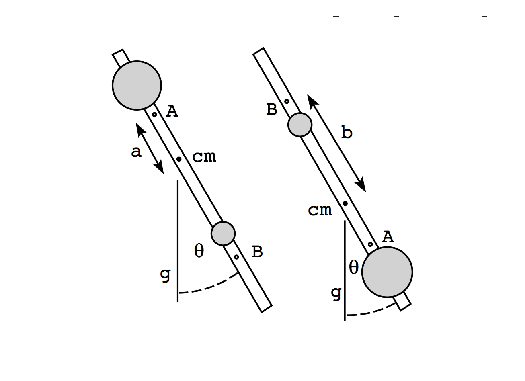
\includegraphics[width=10cm]{katersfig.eps}
\caption{\label{katersfig} 
Kater's pendulum can oscillate about either of the two suspension points
A or B. The two distances $a$ and $b$ are from the center of mass
to the pivot points A and B respectively.}
\end{figure}

For oscillations about point A, the restoring torque on the pendulum of total
mass M is
\begin{equation}
\Gamma_a = -Mga \sin{\theta}
\end{equation}
where $M$ is the total mass of the pendulum and $g$ is the local gravitational
acceleration.  The parallel axis theorem relates the moment of inertia $I_a$
about this pivot point to the moment of inertia about the center of mass of
the system $I_{cm}$ as
\begin{equation}
I_a = I_{cm} + Ma^2 = M(R^2 + a^2)
\end{equation}
where $R = I_{cm}/M$ is defined as the radius of gyration of the pendulum about
its center of mass. Using these quantities, Newton's second law leads to the
following second-order differential equation for the angular displacement
$\theta$
\begin{equation}
I_a\frac{d^2\theta}{dt^2} = -Mga\sin{\theta} 
\end{equation}
where $t$ is time.  For sufficiently small-amplitude oscillations, the factor
$\sin{\theta}$ can be replaced with $\theta$ expressed in radians, which leads
to a simple harmonic equation of motion,
\begin{equation}
\frac{d^2\theta}{dt^2} = -\left(\frac{Mga}{I_a}\right)\theta \label{eq:sho} 
\end{equation}
whose solution is of the general form
\begin{equation}
\theta(t) = \theta_0\sin(\omega t+\delta_0) 
\end{equation}
with integration constants $\theta_0$ and $\delta_0$ to be determined using
information about the initial conditions of the motion.  Substitution of this
solution into Eq.~\eqref{eq:sho} shows that
\begin{equation}
\omega = \left(\frac{Mga}{I_a}\right)^{\frac{1}{2}} 
\end{equation}
or, in terms of the oscillation period $\tau$,
\begin{equation}
\tau_a = 2\pi\left(\frac{R^2+a^2}{ga}\right)^{\frac{1}{2}}
\label{eq:taua} 
\end{equation}
A similar analysis of the oscillations about pivot B gives a period of
\begin{equation}
\tau_b = 2\pi\left(\frac{R^2+b^2}{gb}\right)^{\frac{1}{2}}
\label{eq:taub} 
\end{equation}

These two periods can be measured very precisely by averaging the time
that it takes for the pendulum to undergo many periods of oscillation.
However, in order to use these measurements to extract a value for $g$
from Eqs.~\ref{eq:taua}-\ref{eq:taub}, the values of $a$ and $b$ must also
be known to a comparably high precision.  This would require that the 
position of the center of mass of the system be known, which would be
difficult to determine precisely.  An alternative solution is to adjust
the position of one of the masses, and to make measurements of $\tau_a$
and $\tau_b$ as a function of its position, searching for the point where
the two periods become equal.  One of two conditions must be met in order
for $\tau_a$ to equal $\tau_b$: either $a=b$ or $ab = R^2$.  If the first
possibility can be ruled out -- a crude check shows where the center of mass
is located after the weights have been fixed with the periods approximately
matched -- then the second one must hold.
 
In the configuration with $a\neq b$ where $\tau_a$ and $\tau_b$ share
a common value $\tau_0$,
\begin{eqnarray}
\tau_0^2 &=& \frac{1}{2}(\tau_a^2 + \tau_b^2) \nonumber \\
         &=& \frac{4\pi^2}{2}\left(\frac{R^2+a^2}{ga}+\frac{R^2+b^2}{gb}\right)
                                              \nonumber \\
         &=& \frac{4\pi^2}{2g}\left(\frac{R^2}{a}+a+\frac{R^2}{b}+b\right)
                                              \nonumber \\
         &=& \frac{4\pi^2}{g}\left(a+b\right) 
\end{eqnarray}
Solving for $g$ leads to the final result,
\begin{equation}
g = \left(\frac{2\pi}{\tau_0}\right)^2 L \label{eq:finalresult}
\end{equation}
where $L = a+b$ is the distance between the pivots.



\section{Procedure}
\label{sec:procedure}
Carefully hang the pendulum in its mount, with the edge of the pivot at
position A aligned in the v-groove of the mount.  Allow the pendulum to
swing through 10 periods, using a clock to measure the total time.  The
result you obtain divided by 10 is the approximate period of the pendulum.
A more accurate measurement of the period can be obtained by mounting a
photogate just below the end of the pendulum in its stationary position,
and timing the intervals between the signals produced by the photogate
when the bolt extending from the end of the pendulum interrupts the beam
as it transits through the arms of the photogate.  A computer program has
been set up to record the times between the transits.  The program presents
a graphical window that is used to control the data acquisition and display
results.  To start a run, select the number of periods that you want to
collect and press the Start icon.  Once you set the pendulum swinging,
press the Go arrow to initiate data collection.  Circles are displayed on
the graphical screen every half-period.  If the photogate is positioned
near the neutral position of the pendulum, the two half-period values 
should be approximately the same, but it is not critical that they be
precisely matched.  Take a couple of practice runs and check that the
periods reported by the program are in satisfactory agreement with the
rough estimate you made using the manual method above.  If not, you may
need to adjust with the apparatus until you obtain consistent results.

\begin{figure}
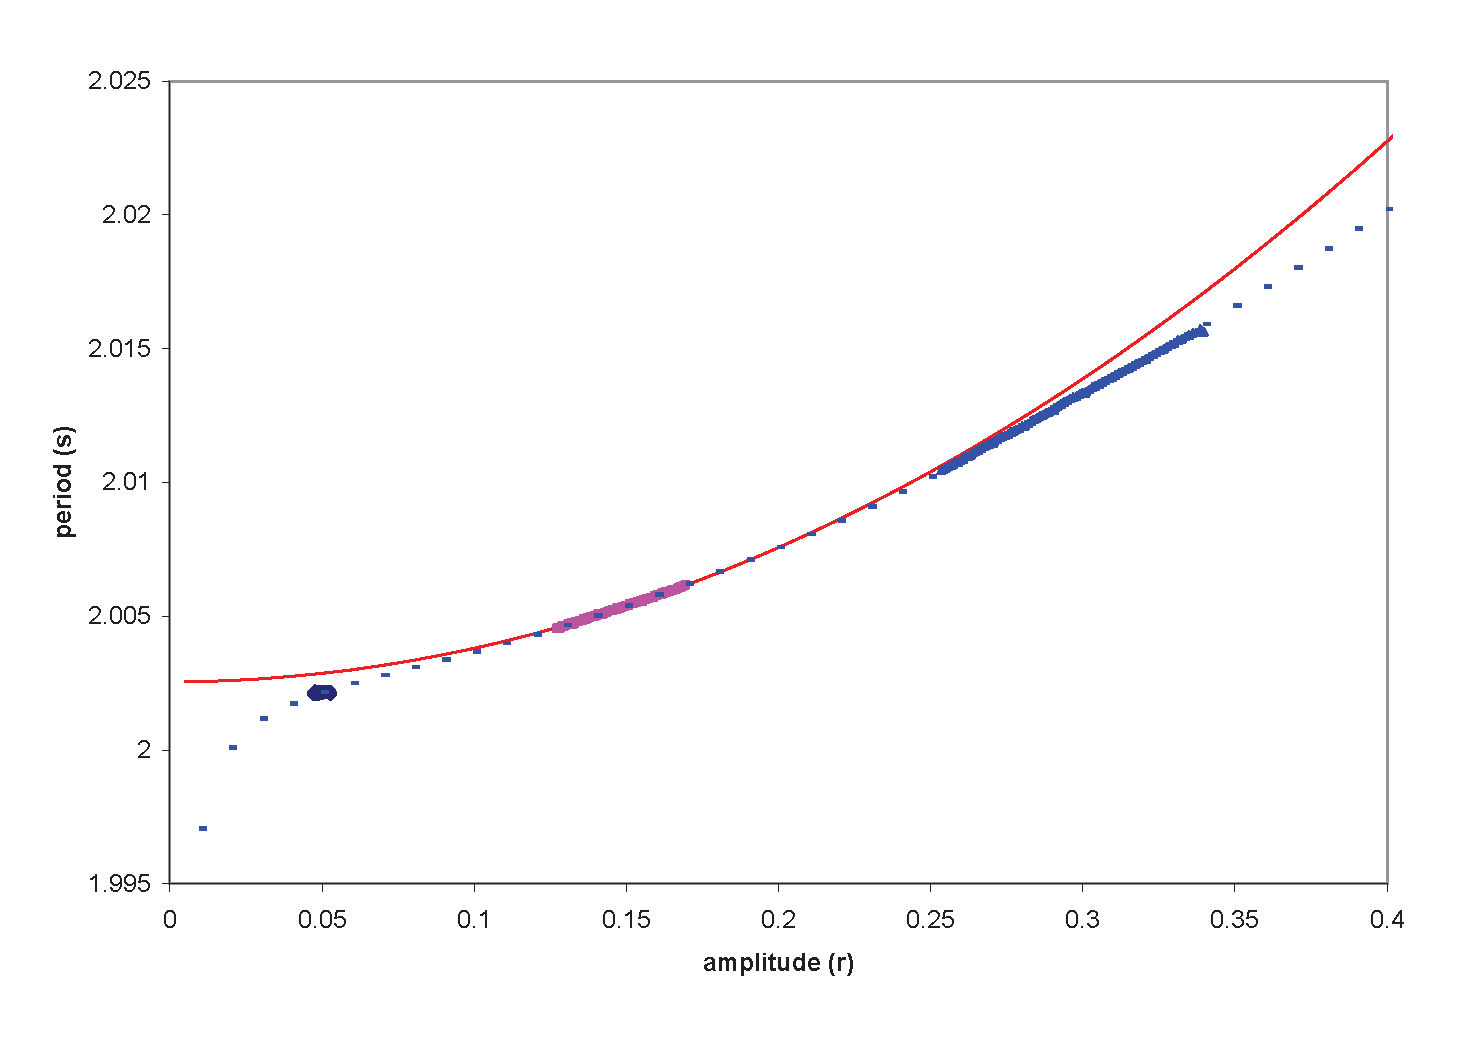
\includegraphics[width=6in]{penduap.eps}
\caption{\label{fig:penduap}
Plot of the measured period of an apparatus similar to the one used in
this experiment, as a function of oscillation amplitude.  The red curve
is the theoretical prediction based on Eq.~\ref{eq:tauofalpha}.  The heavy
solid lines are measurements, and the dashed line is an interpolation
of the measurements over the full dynamic range of the pendulum.
}
\end{figure}

Before beginning to take data for this experiment, you must determine
what is the best amplitude at which to measure the oscillation periods.
Fig.~\ref{fig:penduap} shows an example of several continuous period
measurements taken with an apparatus similar to the one used in this
experiment.  The heavy curve segments are the periods measured with the
photogate, one run at large amplitude, one run at medium amplitude, and
one run at small amplitude.  The dashed curve is an interpolation of these
measurements over the full dynamic range of the pendulum.
Notice that the amplitude damps away during each run, causing the
periods to decrease slightly from the beginning to the end of the run.
Students often find this behavior confusing, and wonder if the apparatus
is defective because the period is changing over time.  There are several
reasons behind this behavior.  The most important reason is that the
period measurements taken with the photogate are so precise that
corrections to the small-angle approximation are required.
The period $\tau$ that you measure at amplitude $\alpha$ is
\begin{equation}
\tau(\alpha) = \tau(0) \left(1+\frac{1}{16}\alpha^2 + \cdots\right)
\label{eq:tauofalpha}
\end{equation}
where $\tau(0)$ is the ideal period you would measure in the small-amplitude
limit.  The terms represented by the ellipsis $(\cdots)$ in
Eq.~\ref{eq:tauofalpha} are higher-order in $\alpha$ and can be ignored
in your analysis.  Eq.~\ref{eq:tauofalpha} is represented by the light
red curve in Fig.~\ref{fig:penduap}.

The reason that you cannot simply
go to tiny amplitudes and get rid of the corrections in Eq.~\ref{eq:tauofalpha}
altogether is seen in Fig.~\ref{fig:penduap} by what happens to the periods
measured with the photogate when the amplitude gets very small.  Imperfections
in the pivot cause tiny restoring forces that act on the pendulum in addition
to gravity.  At very small amplitudes, the gravitational torque on the
pendulum becomes so small that the torques from these tiny pivot
imperfections actually become large enough to compete with gravity and
completely distort the pendulum from its ideal small-angle behavior given
by the red curve.  At very large amplitudes, the sides of the wedge-shaped pivot
start to make contact with the sides of the V-shaped groove in the support.
This creates an additional restoring force that acts on the pendulum at
large amplitudues, in addition to gravity, again reducing the measured
period relative to its ideal value in the presence of gravity alone.

Using Fig.~\ref{fig:penduap} as a guide, choose an initial amplitude that
you will use for your period measurements.  Record its value, together
with the error that comes from how precisely you can determine it.  Each
measurement will be done over a number of oscillation cycles, so the
amplitude will decrease somewhat during the run.  Noting both
the initial and the final amplitude will help you apply
Eq.~\ref{eq:tauofalpha} to your period data and correct them to obtain
the true small-angle period $\tau(0)$.  In reality, the amplitude decreases
exponentially from its initial to its final value, but in practice assuming
that it decreases linearly will introduce a negligible amount of error to
your analysis.

To test different amplitudes, set the photogate program to acquire 50
periods and repeat the run several times at different amplitudes. 
Check that the correction in Eq.~\ref{eq:tauofalpha} gives the same
period $\tau(0)$, independent of amplitude $\alpha$, provided that you
stay within the amplitude range in Fig.~\ref{fig:penduap} where the
red curve coincides with the measurements.

Now take a run with at least 20 periods, and record it as data set A1.
Repeat it at least once to be sure your results are reproducible.  Now
carefully remove the pendulum from its support and replace it so that
it oscillates about the other set of knife edges at pivot B. Do this
gently since these knife edges are delicate. Be sure that the knife edge
is centered in the retaining-groove. Then repeat the period measurements,
calling this data set B1.

Remove the pendulum, rest it on blocks on the bench (not on the
knife edge assembly!) and measure the distance from the near edge of the
large mass to the end of the bar using a vernier caliper.  Record this
value as $x_1$, together with your measurement error $\Delta x_1$.
If you are careful, you should be able to measure $x$ with a precision
of 0.05 mm or better.  Then loosen the large nuts on the large mass and
slide it to a new position, and tighten them again, making sure that the
mass will not slip when the bar is hanging vertically.  Measure the new
distance from the edge of the mass to the end of the bar, and record this
value and its error as $x_2 \pm \Delta x_2$.  Repeat the period
measurements about pivots A and B, labeling the data sets A2 and B2,
respectively.

Based upon how the periods changed between positions $x_1$ and $x_2$,
guess at what value of $x$ the two periods should be approximately the
same, and write that value down as $x_0$.  You will never actually do
a measurement exactly at $x_0$, but it will serve as a reference value
for what follows. Move the large mass to a position close to $x_0$,
then measure it and record its value as $x_3$.
Repeat the two period measurements and record data sets A3 and B3.
If your guess was accurate, they should be much closer than they were
at $x_1$ or $x_2$.  If you guess was off, repeat this process and adjust
the value you assigned to $x_0$ until you are satisfied.  After this,
move to a region in $x$ past $x_0$ where the order of the two periods
is reversed and take another set of measurements.  Repeat this process
for a total of 8-10 values of $x$, with approximately half of them
on each side of $x_0$.  Note that it is not important that you manage
to land exactly on the cross-over point, because it can be determined
with high precision by fitting straight lines to the two sets of data
and solving for the intersection of the two lines.  This procedure is
explained in the next section.

Before the measurement phase of the experiment is completed, be sure to
measure and record the distance $L$ between the two knife edges on the
pendulum.  Use a meter stick for this measurement, and estimate the
error $\Delta L$.  If you are careful, you should be able to do better
than 0.5 mm for $\Delta L$.  A Physics Department machinist has measured
the distance with a precision instrument and written the value on a label
stuck to the side of the pendulum.  You may compare your measurement 
with this marked value, but it may have moved due to handling since the
time the machinist measured it, so your own measurement is the only value
you may use in your analysis.

\section{Data Analysis}

The period data you collected were recorded in run sequences labeled A$i$ and
B$i$ where $i=1..n$.  Examine each run for sag, and select a subset from each
to be used for computing the average, as described in the previous section.
% Compute the combined average period for all of the selected data in a given 
% data set A$i$ or B$i$ and call it $y_{Ai}$ or $y_{Bi}$.
% Compute the RMS
% (root-mean-square) deviation from the mean of the combined data in a given dataset and use that to
% estimate the errors on the individual period measurements. That value
% divided by the square root of the number of individual periods in the data
% set is the error $\Delta y_{Ai}$ or $\Delta y_{Bi}$.
For each run, compute the \emph{average} of all selected period
measurements. Estimate the error in the average period by computing
the standard deviation of the selected data sample and dividing the
result by the square root of the number of measurements included in the
average. Note, however, that this prescription gives a misleading
estimate of the error in the average period, because it assumes that the variations observed in the data are caused
by random errors in the measurement of an unchanging quantity, when in
fact the magnitude of the decrease in period during the run is much
greater than the typical error in a single measurement. 

Use Eq.~\eqref{eq:tauofalpha} to correct the average period from each run using the average amplitude of oscillation to
obtain the ideal small-angle period $\tau(0)$. Estimate the
uncertainty $\Delta \tau(0)$ in the corrected period, keeping in
mind that there is uncertainty not only in the period measurement
itself, but also in the determination of the amplitude.  Knowing the initial ($\alpha_i$) and final ($\alpha_f$)
amplitudes of oscillation for each run, and assuming that the amplitude
decreases linearly with time from
the beginning of the run to the end, a good approximation
to the average amplitude is the average of the initial and final
amplitudes: $\left<\alpha \right> =
\frac{1}{2}\left(\alpha_i + \alpha_f \right)$. Alternatively, if only
the initial amplitude is known, the final amplitude can be estimated
from the ratio of the initial and final periods using $\tau_f/\tau_i \approx
(1+\alpha_f^2)/(1+\alpha_i^2)$, assuming that the
decrease in period from the initial to the final measurement is entirely
explained by deviations from the small-angle approximation. 

% Arrange these in
% 6 adjacent columns in the spreadsheet, with columns labeled $x$, $\Delta x$,
% $y_A$, $\Delta y_A$, $y_B$, and $\Delta y_B$.  Let $x_i=r_i-r_0$ and
% $\Delta x_i=\Delta r_i$.  When you are finished with this, the spreadsheet
% will contain a data block with $6\times n$ values.
% Create a scatter plot with one kind of marker at the points ($x_i$,$y_{Ai}$)
% and a different marker at the points ($x_i$,$y_{Bi}$).  Attach vertical
% error bars to each marker with sizes given by the corresponding  $\Delta y$
% values.  Be sure to adjust the vertical scale of the plot and choose a size
% for the markers that makes the error bars visible.  Label the axes with
% descriptive titles with units as appropriate.  Horizontal errors bars
% depicting the values of $\Delta x_i$ are allowed but not required.
% There should be no lines joining the points.

% Now on top of the scatter plot superimpose two straight lines, one to
% describe how the $y_A$ values vary with $x$ and the other for the $y_B$.
% It helps to choose colors for the lines that match the colors of the data
% markers.  The equations for these lines are
At this point you have a set of corrected periods $\tau_{Ai}(0)$ and
$\tau_{Bi}(0)$ measured at $n$ positions $x_i$ of the larger
mass relative to the end of the bar. To determine the position where $\tau_a$ and $\tau_b$ are equal with $a \ne b$, and the corresponding period $\tau_0$, we must consider the dependence of the periods $\tau_a$ and $\tau_b$ on the position of the large weight near point A.
\begin{figure}[h]
  \begin{center}
    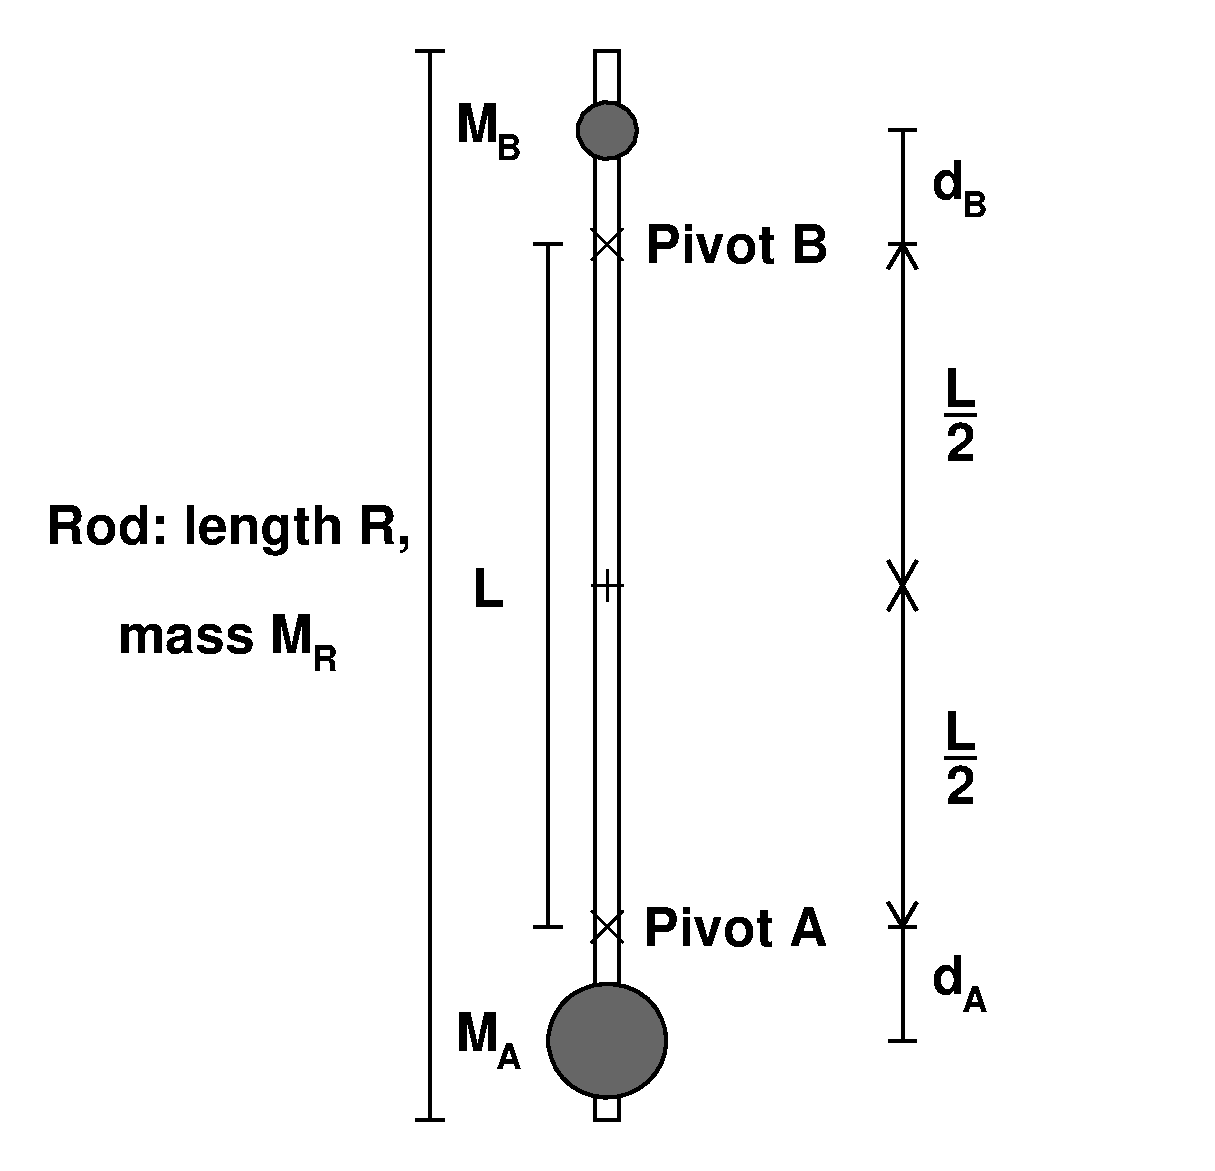
\includegraphics[width=0.4\textwidth]{KatersModelFig.eps}
  \end{center}
  \caption{\label{fig:Katersmodel} Definition of distances and masses in a simplified model of the Kater's pendulum apparatus. The bar is approximated as a thin rod of length $R$ with mass $M_R$ and uniform density. Pivot points A and B are assumed equidistant from the ends of the rod, such that the midpoint between A and B coincides with the midpoint of the rod. $M_A$ and $M_B$ are assumed to be point masses. The masses satisfy $M_A > M_B$, and the distances satisfy $0 \le d_{A,B} \le \frac{R-L}{2}$.}
\end{figure} 
Figure~\ref{fig:Katersmodel} shows a simple model for calculating the period of Kater's pendulum. Assume that the rigid bar is a thin rod of total length $R$ and mass $M_R$ with uniform density. Then assume that the pivot points A and B are equidistant from the ends of the rod, so that the midpoint between A and B coincides with the midpoint of the rod. This assumption is not crucial, but it simplifies the algebra. Finally, assume that the weights A and B at either end are point masses at a distance $\frac{L}{2} + d_{A,B}$ from the midpoint of the rod. Define the origin of coordinates as the midpoint of the rod, with the positive $x$ direction pointing from A toward B. In this coordinate system, the position of the center of mass is given by: 
\begin{eqnarray}
  M x_{CM} &=& M_B (d_B + \frac{L}{2}) - M_A (d_A + \frac{L}{2} ) \nonumber \\
  x_{CM} &=& \frac{M_B}{M} d_B + \frac{M_B -M_A}{M}\frac{L}{2} - \frac{M_A}{M}d_A \label{eq:xCM} \\ 
  M &\equiv& M_A + M_B + M_R \nonumber 
\end{eqnarray}
From Eq.~\eqref{eq:xCM}, we see that the position of the center of mass is a linear function of $d_A$. It is assumed that the relationships among the various masses and distances are such that the position of the center of mass lies between A and B; i.e., $-\frac{L}{2} \le x_{CM} \le \frac{L}{2}$. The distances from each pivot to the center of mass are given by
\begin{eqnarray}
  a &=& x_{CM} + \frac{L}{2} = \frac{M_B}{M} d_B + \frac{M_B - M_A + M}{M}\frac{L}{2} - \frac{M_A}{M} d_A \nonumber \\
  b &=& \frac{L}{2} - x_{CM} = -\frac{M_B}{M}d_B + \frac{M_A - M_B + M}{M} \frac{L}{2} + \frac{M_A}{M} d_A
\end{eqnarray}

Under the assumption that pivot points A and B are equidistant from the ends of the rod, the moment of inertia of the rod about either pivot point is 
\begin{eqnarray}
  I_R &=& I_0^R + \frac{M_RL^2}{4} \nonumber \\
  I_0^R &=& \frac{M_R}{R}\int_{-\frac{R}{2}}^{\frac{R}{2}} x^2 dx = \frac{M_R R^2}{12} \nonumber \\
  I_R &=& \frac{M_R}{4}\left[L^2 + \frac{R^2}{3}\right]
\end{eqnarray}
With the additional point masses included, the total moments of inertia for oscillations about pivot points A and B are given by
\begin{eqnarray}
  I_a &=& I_R + M_A d_A^2 + M_B (d_B + L)^2 \nonumber \\
  I_b &=& I_R + M_A (d_A + L)^2 + M_B d_B^2, 
\end{eqnarray}
from which we see that $I_a$ and $I_b$ are quadratic functions of $d_A$.
\begin{figure}[h]
  \begin{center}
    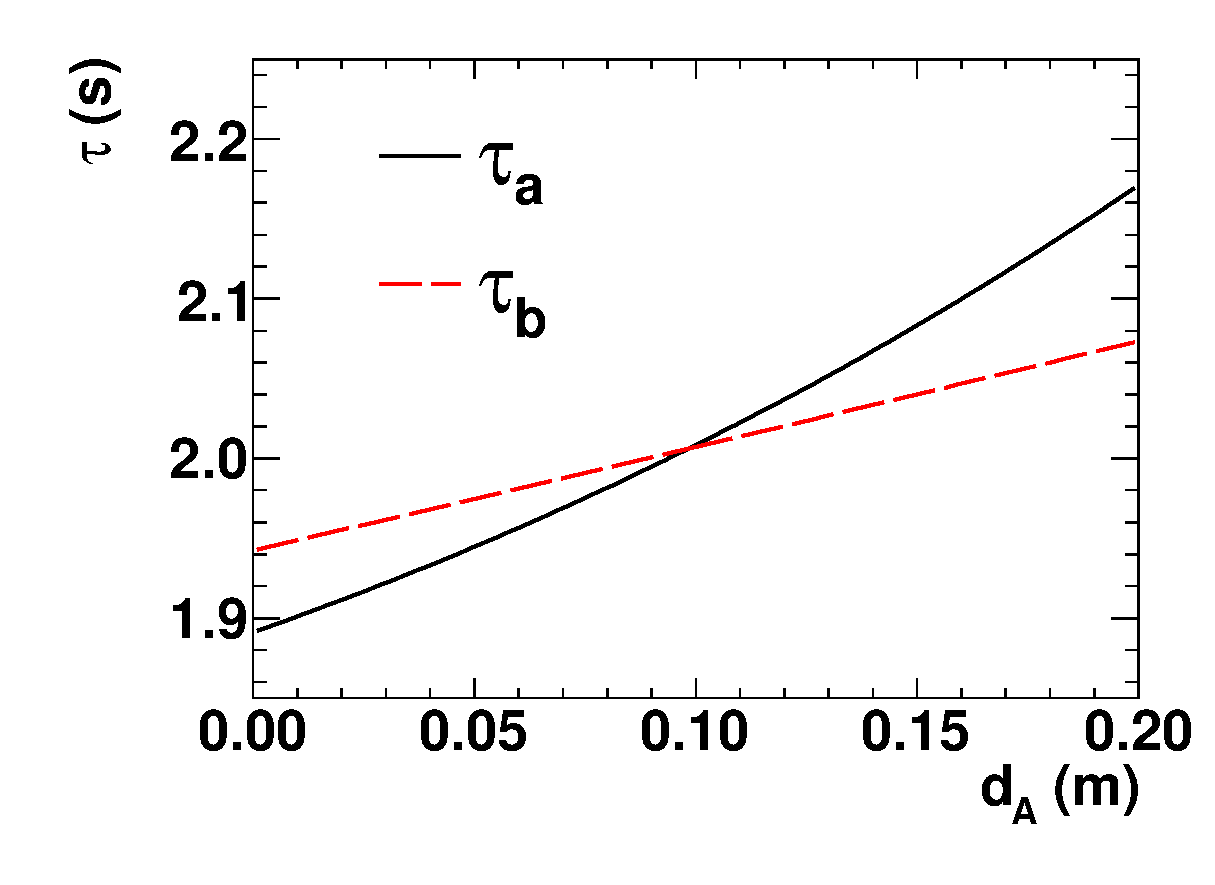
\includegraphics[width=0.4\textwidth]{KatersModelFig2.eps}
  \end{center}
  \caption{\label{fig:Katers_model_predict} Oscillation periods $\tau_a$ and $\tau_b$ as a function of the distance $d_A$ from pivot A to the larger weight, calculated from the simplified model of Fig.~\ref{fig:Katersmodel}, assuming $L = 1$ m, $R = 1.4$ m, $M_A = 2$ kg, $M_B = 0.4$ kg, $M_R = 3$ kg and $d_B = 10$ cm. Note that these calculations are illustrative only, and the model parameters assumed do \emph{not} necessarily coincide with the apparatus you used.}
\end{figure}
Figure~\ref{fig:Katers_model_predict} shows the prediction of this model for the dependence of $\tau_a$ and $\tau_b$ on the distance $d_A$ from the pivot point to the position of the larger weight, assuming masses and dimensions similar (but not identical) to the pendulum you will actually use. In general, $\tau_a$ and $\tau_b$ vary non-linearly with $d_A$ (which is related to the distance $x$ that you measured). However, if the analysis is confined to a sufficiently narrow range surrounding the intersection point between the two curves, the deviations from linearity can be ignored, and the intersection point can be located by fitting straight lines to the $x$ dependence of the corrected periods $\tau_{Ai}(0)$ and $\tau_{Bi}(0)$ in the vicinity of the intersection point.

Assuming that $y_{A,Bi} \equiv \tau_{A,Bi}(0)$ depends linearly on $x_i$, determine the slope and intercept parameters $(m_A, t_A)$ and $(m_B, t_B)$ describing the lines of best fit through the data sets $(x_i,y_{Ai})$ and $(x_i,y_{Bi})$:
\begin{eqnarray}
y_A(x) &=& m_A x + t_A \label{eq:lineA} \\
y_B(x) &=& m_B x + t_B \label{eq:lineB}
\end{eqnarray}
Define a $\chi^2$ statistic for data set A, and a separate one for data
set B, comparing the above linear formulas with your measured values for
the period of the pendulum.  The $\chi^2$ statistic is defined as
\begin{equation}
\chi^2 = \sum_{i=1}^N\left(\frac{y_i-y(x_i)}{\Delta y_i}\right)^2
\end{equation}
The best-fit values for the unknown parameters $m_A$, $t_A$, $m_B$ and $t_B$ are determined by minimizing the $\chi^2$ for each data set as a function of these parameters. In the general least-squares problem where data are fitted to an arbitrary function $y = y(x;p_i,i=1,\ldots,m)$ depending on $m$ parameters $p_i$ to be optimized, $\chi^2$ is minimized by solving the $m$ simultaneous equations $\partial \chi^2/\partial p_i = 0, i=1,\ldots,m$. One of the by-products of this procedure is the {\em error matrix} that describes the uncertainties and correlations among the best-fit parameters. The diagonal elements of the error matrix give the variances of the parameters ($\mathcal{E}_{ii} \equiv \sigma^2_{p_i}$), while the off-diagonal elements give the covariances between parameters ($\mathcal{E}_{ij} \equiv \mbox{cov}(p_i,p_j), i \ne j$). The inverse of the error matrix $\mathcal{E}$ for the general least-squares problem is approximately given by the following matrix of second partial derivatives of $\chi^2$ with respect to the parameters $p_i$ and $p_j$, evaluated at the function minimum:
\begin{eqnarray}
  \mathcal{E}^{-1}_{ij} &=& \frac{1}{2} \frac{\partial^2 \chi^2}{\partial p_i \partial p_j} \label{Hessian}
\end{eqnarray}
The matrix of partial derivates in equation~\eqref{Hessian}, often called the ``Hessian'', is simply the matrix of coefficients of the quadratic terms of order $(p_i - \hat{p}_i)(p_j - \hat{p}_j)$ in the Taylor expansion of $\chi^2$ about the local minimum corresponding to the best-fit values of the parameters (denoted by $\hat{p}_i$). For any $\chi^2$ in which the fit function $y(x; p_i)$ is a \emph{linear} function of the parameters $p_i$, equation~\eqref{Hessian} for the error matrix is \emph{exact}, since all higher derivatives vanish. 

Now suppose we have performed a fit and determined the best-fit values of several parameters along with their error matrix, and we want to compute the error on a function $f(p_i)$ of the parameters. We treat the parameter errors as random variables whose variances and covariances are sufficiently ``small'' that we can approximate the function $f$ in the vicinity of the best-fit values of its parameters by its first-order Taylor expansion:
\begin{eqnarray}
  df &=& \sum_{i=1}^{n} \frac{\partial f}{\partial p_i} dp_i \label{eq:Taylor1},
\end{eqnarray}
As usual, the partial derivatives are evaluated using the best-fit parameter values. We are interested in the \emph{variance} (standard deviation squared) of $f$, so we square Eq.~\eqref{eq:Taylor1} and take its ``expectation value'' (denoted $\left<\ldots\right>$), which is the average of $(df)^2$ over the hypothetical distribution of an infinite number of similar experiments in which the ``best-fit'' value of $f$ varies randomly in response to random variations in the parameters due to experimental errors:   
\begin{eqnarray}
  \left<(df)^2\right> &=& \sum_{i=1}^{n}\sum_{j=1}^n \left(\frac{\partial f}{\partial p_i}\right)\left(\frac{\partial f}{\partial p_j}\right)\left<dp_i dp_j\right> \nonumber \\
  \sigma_f^2 &=& \sum_{i=1}^{n}\sum_{j=1}^n \left(\frac{\partial f}{\partial p_i}\right)\left(\frac{\partial f}{\partial p_j}\right) \mathcal{E}_{ij}, \label{errorpropagation}
\end{eqnarray}
where on the second line the expectation value $\left<dp_i dp_j\right>$ has been replaced by the error matrix element $\mathcal{E}_{ij}$. 

The error
matrix from a linear least-squares fit is a 2x2 matrix $\cal{E}$ of the
following form.
\begin{equation}
\cal{E} = \left(\begin{array}{cc}
V_m & C_{mt} \\
C_{mt} & V_t
\end{array}\right)
\end{equation}
where $V_m$ is the variance (standard deviation squared) on the best-fit
value of $m$, $V_t$ is the variance on the best-fit value of $t$, and
$C_{mt}$ is their covariance.

With estimates for $m_A,t_A$ and $m_B,t_B$ and their error matrices in hand,
it is time to solve for the intersection of the two lines.  For the purposes
of this experiment, only the $y$-value at the intersection is needed, not the
$x$-value. Denote the estimated value of $y$ at the intersection as $y_0$ and its error as $\Delta y_0$.
\begin{equation}
y_0 = \frac{m_At_B-m_Bt_A}{m_A-m_B} \label{eq:intersect}
\end{equation}
To find the error on $y_0$, we invoke the general prescription for the propagation of uncertainties and correlations from random variables to functions of those variables as described above, recalling that there are covariances between $m_A$ and $t_A$, and between
$m_B$ and $t_B$, but the covariances between the parameters describing data sets A and B are zero.
Apply the principle given in Eq.~\ref{errorpropagation} to obtain the variance on the value $y_0$ obtained using
Eq.~\ref{eq:intersect}. The error $\Delta y_0$ is the square root of
the variance.

The final analysis step is to extract an estimate $\hat{g}$ for the local
value of $g$ and its error $\Delta \hat{g}$.  In terms of the quantities
defined above, these are
\begin{equation}
\hat{g} = \left(\frac{2\pi}{y_0}\right)^2L
\end{equation}
\begin{equation}
\Delta \hat{g} = \hat{g}\sqrt{4\left(\frac{\Delta y_0}{y_0}\right)^2
+\left(\frac{\Delta L}{L}\right)^2}
\end{equation}

\section{Interpretation}
The value of the local acceleration of gravity varies with
latitude $\varphi$ and elevation above sea level $h$.  One common
approximation~\cite{Heiskanen67,Geodesy71} for this dependence is
\begin{equation}
g = g_0\left(1 + A\sin^2{\varphi} - B\sin^2{2\varphi} - Ch\right)
\end{equation}
where $g_0$ = 9.78031846 m/s$^2$, $A = 5.3024\times 10^{-3}$, 
$B = 5.8\times 10^{-6}$, and $C = 3\times 10^{-7}$ m$^{-1}$.
Evaluate this formula for $g$ at the location of Storrs, Connecticut and
compare this value to the one that you have measured.

\begin{acknowledgments}
This document was updated by Prof. Richard Jones and Prof. Andrew Puckett, based on an original 
write-up by Prof. Doug Hamilton, University of Connecticut, 1988.
\end{acknowledgments}

\appendix
\section{Finite-amplitude correction}
\label{appendixA}
As described in Section~\ref{sec:procedure}, the photogate apparatus you used to measure the
oscillation period of the pendulum is sufficiently precise that
deviations from the small-angle approximation are not small compared
to the uncertainty in the measurement. At the leading order in
$\alpha$, the amplitude-dependence of the period is given by
Eq.~\eqref{eq:tauofalpha}. Equation~\eqref{eq:tauofalpha} can be
derived by considering energy conservation for oscillations about pivot point $a$ (identical
considerations apply to oscillations about pivot point $b$). If the
pendulum is released from rest at a starting angle of $\alpha$, its
gravitational potential energy relative to the pivot point is
\begin{eqnarray}
  U &=& -M g a \cos \alpha
\end{eqnarray}
As the pendulum oscillates, the sum of its kinetic and potential
energies is conserved, implying that the following equation is valid
for \emph{any} $\theta$:
\begin{eqnarray}
  -M g a \cos \alpha &=& -M g a \cos \theta + \frac{1}{2} I_a
  \left(\frac{d\theta}{dt}\right)^2, 
\end{eqnarray}
leading to the following differential equation for the angular
velocity $\frac{d\theta}{dt}$:
\begin{eqnarray}
  \left(\frac{d\theta}{dt}\right)^2 &=& \frac{2Mga}{I_a}\left(\cos
    \theta - \cos \alpha \right) = 2\omega_a^2 \left(\cos
    \theta - \cos \alpha\right)
\end{eqnarray}
This equation can be rewritten as:
\begin{eqnarray}
  \frac{dt}{d\theta} &=& \frac{\tau_a}{2\pi \sqrt{2(\cos \theta - \cos \alpha)}} \label{dteq},
\end{eqnarray}
where $\tau_a = 2\pi/\omega_a$ is the oscillation period
in the limit $\alpha \rightarrow 0$. To obtain the finite-amplitude period $\tau_a(\alpha)$, we integrate
Eq.~\eqref{dteq} over one quarter-cycle of oscillation (each
half-swing of the pendulum takes the same amount of time) and multiply by
four:
\begin{eqnarray}
  \tau_a(\alpha) &=& \frac{2\tau_a}{\pi\sqrt{2}} \int_{0}^{\alpha}
  \frac{d\theta}{\sqrt{\cos \theta - \cos \alpha} }
\end{eqnarray} 
Noting that $\cos x = 1 - 2\sin^2 \frac{x}{2}$, we can rewrite the
integral as
\begin{eqnarray}
  \tau_a(\alpha) &=& \frac{2\tau_a}{\pi\sqrt{2}} \int_{0}^{\alpha}
  \frac{d\theta}{\sqrt{2(\sin^2 \frac{\alpha}{2} - \sin^2
      \frac{\theta}{2} )}} = \frac{\tau_a k}{\pi}
  \int_{0}^{\alpha} \frac{d\theta}{\sqrt{1-k^2 \sin^2
      \frac{\theta}{2}}}, k \equiv \frac{1}{\sin \frac{\alpha}{2}}.
\end{eqnarray}
By making the substitution $\sin u = k \sin (\theta/2)$, the integral
can be rewritten as
\begin{eqnarray}
  \tau_a(\alpha) &=& \frac{2 \tau_a}{\pi} \int_{0}^{\pi/2}
  \frac{du}{\sqrt{1-\sin^2 u \sin^2 \frac{\alpha}{2}}} \label{Tint_exact}
\end{eqnarray}
The integral in Eq.~\eqref{Tint_exact} can be approximated by
Taylor-expanding the integrand for small but non-zero values of $\alpha$:
\begin{eqnarray} 
  \sin^2 \frac{\alpha}{2} &\approx& \frac{\alpha^2}{4}\nonumber \\
  \frac{1}{\sqrt{1-\sin^2 u \sin^2 \frac{\alpha}{2}}} &\approx & 1 +
  \frac{\alpha^2}{8} \sin^2 u. \label{integrand_LO} 
\end{eqnarray}
Substituting the approximate expression \eqref{integrand_LO} into the
exact equation~\eqref{Tint_exact}, we obtain 
\begin{eqnarray}
  \tau_a(\alpha) &\approx& \frac{2\tau_a}{\pi} \int_{0}^{\pi/2} \left[1 + \frac{\alpha^2}{8}
  \sin^2 u \right]du = \tau_a \left[ 1 + \frac{ \alpha^2}{16}
\right]. \label{finiteamplitudecorrection},
\end{eqnarray}
thus recovering equation~\eqref{eq:tauofalpha}. In going beyond the small-angle approximation, the pendulum's motion
is no longer simple harmonic, and the period of oscillation depends on
the amplitude $\alpha$. At the leading order in $\alpha$, the period
increases by the factor $1 + \alpha^2/16$, a small but noticeable
correction in this experiment as pointed out in section~\ref{sec:procedure}.

%% Create the reference section using BibTeX:
%\bibliography{revtex4}

\begin{thebibliography}{9}

\bibitem{Symon71}
 Keith R. Symon,
 \emph{Mechanics},
 Addison-Wesley, Reading MA, 
 3rd ed. (1971) pp. 214-215.

\bibitem{Kleppner73}
 D. Kleppner and R.J. Kolenkow,
 \emph{An Introduction to Mechanics},
 McGraw-Hill, New York,
 (1973) pp. 257-257.

\bibitem{Marion95}
 J.B. Marion,
 \emph{Classical Dynamics of Particles and Systems},
 Sanders, Fort Worth,
 4th ed. (1995) p. 455.

\bibitem{Heiskanen67}
 W.A. Heiskanen, and H. Moritz,
 \emph{Physical Geodesy},
 W.H. Freeman, San Francisco
 (1967).

\bibitem{Geodesy71}
 International Association of Geodesy,
 \emph{Geodetic Reference System 1967},
 Publi. Sp\'{e}c. no. 3 du Bulletin G\'{e}od\'{e}sique, Paris,
 (1971).

\end{thebibliography}

\end{document}
%%
%% ****** End of file template.aps ******
%
%
